\documentclass[11pt]{article}

\usepackage[left=1.5cm, right=1.5cm, top=2cm, bottom=2cm]{geometry}
\usepackage{amsmath}
\usepackage{amssymb}
\usepackage{amsfonts}
\usepackage{physics}
\usepackage{booktabs}
\usepackage{graphicx}
\usepackage{subcaption}
\usepackage{float}
\usepackage{bm}

\title{t2g square lattice tight-binding derivation}
\author{Anderson Steckler}
\date{}

\begin{document}
\maketitle

\section{Single Layer}
\noindent
We look at hopping from all orbitals along the two x-y directions.
\subsection{xy band}
\subsubsection{x-direction}
\begin{figure}[H]
    \centering
    \begin{subfigure}[b]{0.32\textwidth}
        \centering
        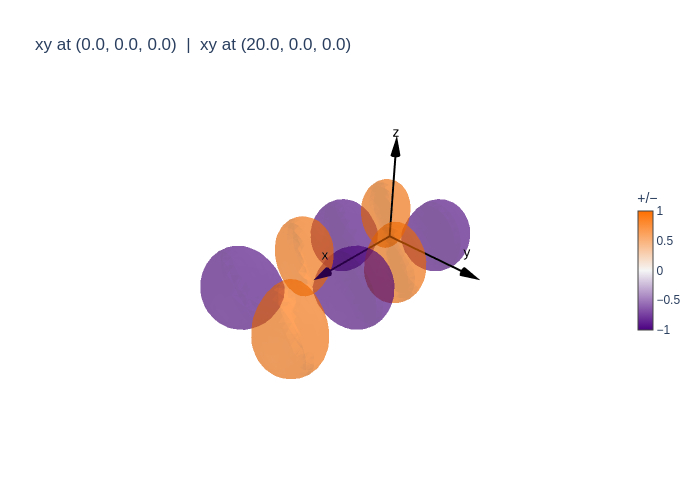
\includegraphics[width=\textwidth]{images/xshift_xy_xy.png}
        \caption{$d_{xy}$--$d_{xy}$}
    \end{subfigure}
    \hfill
    \begin{subfigure}[b]{0.32\textwidth}
        \centering
        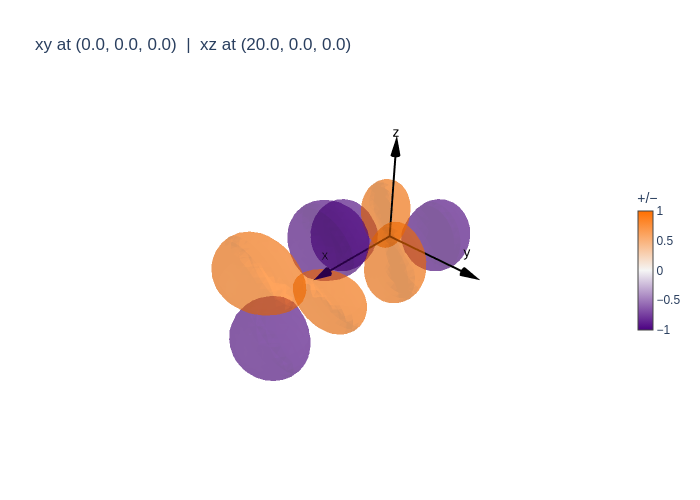
\includegraphics[width=\textwidth]{images/xshift_xy_xz.png}
        \caption{$d_{xy}$--$d_{xz}$}
    \end{subfigure}
    \hfill
    \begin{subfigure}[b]{0.32\textwidth}
        \centering
        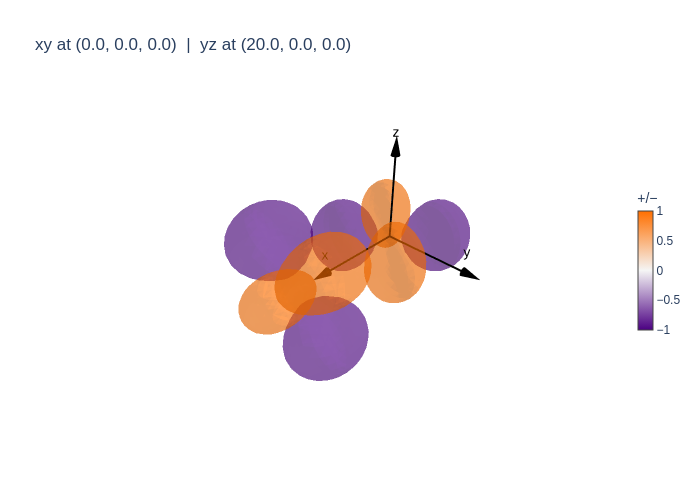
\includegraphics[width=\textwidth]{images/xshift_xy_yz.png}
        \caption{$d_{xy}$--$d_{yz}$}
    \end{subfigure}
    \caption{t2g orbital overlaps for nearest-neighbour hopping along $x$.}
    \label{fig:xshift_overlaps}
\end{figure}

We look at the slater-koster integrals. The slater direction cosines are
\begin{gather}
    l = \frac{\bm R \cdot \hat x}{|\bm R|} \quad m = \frac{\bm R \cdot \hat y}{|\bm R|} \quad n = \frac{\bm R \cdot \hat z}{|\bm R|} \\
\end{gather}
In the x direction this is just.
\begin{gather}
    l = 1 \quad m = 0 \quad n = 0
\end{gather}
This simplifies the xy-xy, xy-xz, and xy-yz integrals to
\begin{gather}
    t_{xy,xy} = V_{dd\pi} \quad
    t_{xy,yz} = 0 \quad
    t_{xy,xz} = 0
\end{gather}

\subsubsection{y-direction}
\begin{figure}[H]
    \centering
    \begin{subfigure}[b]{0.32\textwidth}
        \centering
        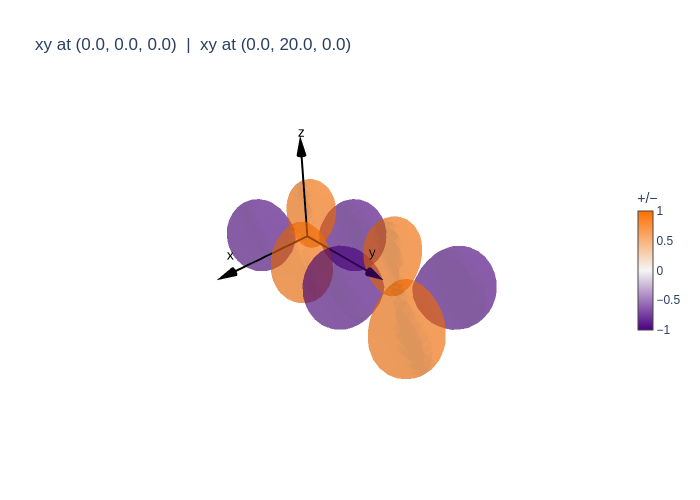
\includegraphics[width=\textwidth]{images/yshift_xy_xy.png}
        \caption{$d_{xy}$--$d_{xy}$}
    \end{subfigure}
    \hfill
    \begin{subfigure}[b]{0.32\textwidth}
        \centering
        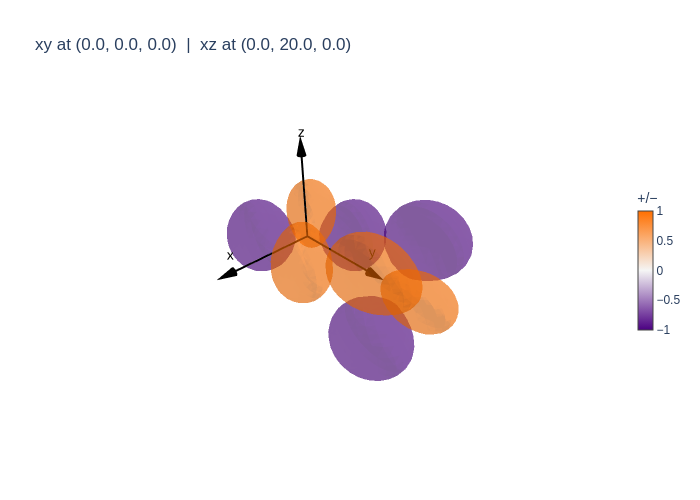
\includegraphics[width=\textwidth]{images/yshift_xy_xz.png}
        \caption{$d_{xy}$--$d_{xz}$}
    \end{subfigure}
    \hfill
    \begin{subfigure}[b]{0.32\textwidth}
        \centering
        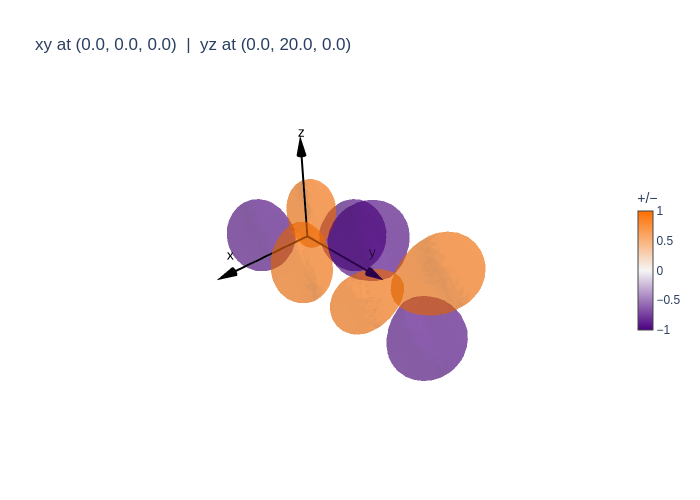
\includegraphics[width=\textwidth]{images/yshift_xy_yz.png}
        \caption{$d_{xy}$--$d_{yz}$}
    \end{subfigure}
    \caption{t2g orbital overlaps for nearest-neighbour hopping along $y$.}
    \label{fig:yshift_overlaps}
\end{figure}
For the y-direction the slater direction cosines are
\begin{gather}
    l = 0 \quad m = 1 \quad n = 0
\end{gather}
and the integrals are
\begin{gather}
    t_{xy,xy} = V_{dd\pi} \quad
    t_{xy,yz} = 0 \quad
    t_{xy,xz} = 0
\end{gather}
\subsubsection{Tight Binding Hamiltonian}
Putting this all together we get this hopping term in the hamiltonian and apply the Fourier transformation
$c_i = \frac{1}{\sqrt{N}} \sum_k e^{i \bm k \cdot \bm R_i} c_{\bm k}$
\begin{align}
    H &= t \sum_{R, \delta} c_{i+\delta}^\dagger c_i \\\nonumber
    &= \frac{t}{N} \sum_{R, \delta} \sum_{q, k} e^{-i \bm q \cdot (\bm R_i + \bm \delta)} e^{i \bm k \cdot \bm R_i} c_{\bm q}^\dagger c_{\bm k} \\\nonumber
    &= \frac{t}{N} \sum_\delta \sum_{q, k} \delta_{qk} e^{-i \bm q \cdot \bm \delta} c_q^\dagger c_k \\\nonumber
    &= t \sum_\delta \sum_k e^{-i q \cdot \delta} c_k^\dagger c_k \\\nonumber
    &= t\sum_k \left[e^{-ik_x a} + e^{-ik_y a} + e^{ik_x a} + e^{ik_y a}\right]c_k^\dagger c_k \\\nonumber
    &= 2V_{dd\pi} \sum_k \left[\cos(k_x a) + cos(k_y a)\right]c_k^\dagger c_k
\end{align}
\subsubsection{Next Nearest Neighbor Hopping}
Now lets consider this one for the xy band. The hopping vector is now $(a \hat x + a \hat y)$. Our directional cosines are
\begin{gather}
    l = 1/\sqrt{2} \quad m = 1/\sqrt{2} \quad n = 0
\end{gather}
and the non zero integrals are
\begin{gather}
    t_{xy-xy} = \frac{3}{4} V'_{dd\sigma} + \frac{1}{4} V'_{dd\delta}
\end{gather}
where the primes denote NNN integrals. It turns out this is the result for all directions i.e $(\pm a \hat x + \pm a \hat y)$ our
tight binding hamiltonian can then be written as.
\begin{align}
    H &= t_{nnn} \sum_\delta \sum_k e^{-ik \cdot \delta} c_k^\dagger c_k \\\nonumber
    &= t_{nnn} \sum_k \left[e^{-ia(k_x+k_y)}+e^{-ia(k_x-k_y)}+e^{-ia(-k_x+k_y)} + e^{-ia(-k_x-k_y)}\right] c_k^\dagger c_k \\\nonumber
    &= t_{nnn} \sum_k \left[2\cos(k_xa + k_ya) + 2\cos(k_xa - k_ya)\right] c_k^\dagger c_k \\\nonumber
    &= 4t_{nnn} \sum_k \cos(k_x a)\cos(k_y a) c_k^\dagger c_k \\\nonumber
\end{align}
Using the sum to product $\cos(A + B) + \cos(A - B) = 2\cos A \cos B$
\subsubsection{Energy for Band}
Hence the total energy for the xy band is
\begin{gather}
    \varepsilon_{xy} = -2t_1 \left[\cos(k_x a) + \cos(k_y a)\right] - 4 t_2 \cos(k_x a)\cos(k_y a)
\end{gather}
\subsection{yz band}
To look at the yz band we apply the following permutation. Its helpful to look at this diagram
\begin{figure}[H]
    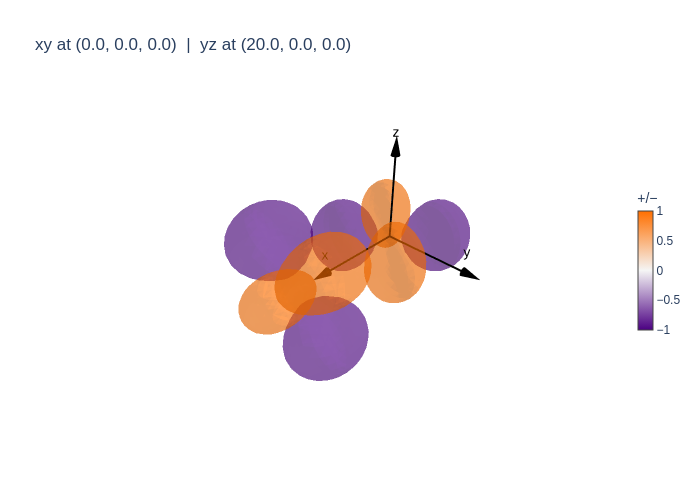
\includegraphics[width=0.5\textwidth]{images/xshift_xy_yz.png}
\end{figure}
From xy we get yz by permuting the axis like $x\xrightarrow{} y \xrightarrow{} z\xrightarrow{}x$, which means
our direction cosines become $l\xrightarrow{} m \xrightarrow{} n\xrightarrow{}l$
\subsubsection{x direction}
\begin{gather}
    l = 0 \quad m = 1 \quad n = 0
\end{gather}
\begin{gather}
    t_{yz,yz} = V_{dd\pi} \quad
    t_{yz,xy} = 0 \quad
    t_{yz,xz} = 0
\end{gather}
The hamiltonian is
\begin{align}
    H &= t\sum_\delta \sum_k e^{-ik\cdot \delta} c^\dagger_k c_k \\\nonumber
    &= t \sum_k \left[e^{-ik_xa} + e^{ik_xa}\right] c^\dagger_k c_k \\\nonumber
    &= 2V_{dd\pi} \sum_k \cos(k_x a) c^\dagger_k c_k
\end{align}
\subsubsection{y direction}
\begin{gather}
    l = 0 \quad m = 0 \quad n = 1
\end{gather}
\begin{gather}
    t_{yz,yz} = V_{dd\delta} \quad
    t_{yz,xy} = 0 \quad
    t_{yz,xz} = 0
\end{gather}
The derivation for the energy is the same as above just in y direction.
\subsubsection{Next Nearest Neighbor Hopping}
We do the permutation to the directional cosines in the xy case to get
\begin{gather}
    l = 0 \quad m = \pm 1/\sqrt{2} \quad n = \pm 1/\sqrt{2}
\end{gather}
the diagonal hopping term is
\begin{gather}
    t_{yz,yz} = \frac{1}{2} V'_{dd\pi} + \frac{1}{2} V'_{dd\delta}
\end{gather}
which is the same for all diagonal directions so this gives us an additional diagonal term
\begin{gather}
    \varepsilon_{yz, nnn} = -4t_{yz,yz} \cos(k_x a)\cos(k_y a)
\end{gather}
Now the off diagonal gives us $t_{yz, xz} = 0$ but a nonzero
\begin{gather}
    t_{yz, xy} = \pm \frac{1}{2} \left[V'_{dd\pi} - V'_{dd\delta}\right]
\end{gather}
where it is plus/minus depending on the product of the direction cosines, i.e in our
hopping hamiltonian we see
\begin{align}
    H &= t_{yz,xy} \sum_\delta \sum_k e^{-ik \cdot \delta} c_k^\dagger c_k \\\nonumber
    &= t_{yz,xy} \sum_k \left[e^{-ia(k_x+k_y)}-e^{-ia(k_x-k_y)}-e^{-ia(-k_x+k_y)} + e^{-ia(-k_x-k_y)}\right] c_k^\dagger c_k \\\nonumber
    &= t_{yz,xy} \sum_k 2i \left[\sin(k_x + k_y) + \sin(k_x - k_y)\right] c_k^\dagger c_k \\\nonumber
    &= 4i t_{yz,xy} \sum_k \sin(k_x a) \cos(k_y a) c_k^\dagger c_k
\end{align}
\subsection{Energy for band}
Hence the total energy is
\begin{gather}
    \varepsilon_{yz} = -2t_1 \cos(k_x a) - 2 t_\delta \cos(k_y a) \\
    \langle yz| H_0 | xy \rangle = -4i t_{yz,xy} \sin(k_x a) \cos(k_y a)
\end{gather}
\subsection{xz band}
The same formalism applies.
\subsection{x dir}
\begin{gather}
    l = 0 \quad m = 0 \quad n = 1
\end{gather}
which gives the nonzero integral $V_{dd\delta}$
\subsection{y dir}
\begin{gather}
    l= 1 \quad m= 0 \quad n=0
\end{gather}
which gives the nonzero integral $V_{dd\pi}$.
\subsection{Next Nearest Neighbor Hopping}
The directional cosines are
\begin{gather}
    l= 1/\sqrt{2} \quad m = 0 \quad n = 1/\sqrt{2}
\end{gather}
\subsection{Energy For Band}
\begin{gather}
    \varepsilon_{xz} = -2t_\delta \cos(k_x a) - 2 t_1 \cos(k_y a)
\end{gather}
\subsection{Summary}
\begin{align*}
    \varepsilon_{xy} &= -2t_1 \left[\cos(k_x a) + \cos(k_y a)\right] - 4 t_2 \cos(k_x a)\cos(k_y a) \\
    \varepsilon_{yz} &= -2t_1 \cos(k_x a) - 2 t_\delta \cos(k_y a) \\
    \varepsilon_{xz} &= -2t_\delta \cos(k_x a) - 2 t_1 \cos(k_y a)
\end{align*}    
\end{document}